%%% Laboratory	 Notes
%%% Template by Mikhail Klassen, April 2013
%%% Contributions from Sarah Mount, May 2014
%%% Updated by Muhammad Davi, September 2022
\documentclass[a4paper]{tufte-handout}
\usepackage{lab_notes}

\title{Practice Big Data}
\date{2022}

\begin{document}
\maketitle

%%%%%%%%%%%%%%%%%%%%%%%%%%%%%%%%%%%%%%%%%%%%%%%%%%%%%%%%

\begin{projects}
	\begin{description}
		\item [Muhammad Davi, S.Kom., M.Cs.] adalah sebagai dosen pengampu matakuliah practice big data\footnote{Dosen Prodi Teknologi Rekayasa Komputer Jaringan, Jurusan Teknologi Informasi dan Komputer, Politeknik Negeri Lhokseumawe}.
		\item [Peserta dan Kelompok] matakuliah practice big data adalah sebegai berikut:

\begin{table}[!ht]
\caption{Peserta dan Kelompok Matakuliah Practice Big Bata}
\label{tab:peserta}
\centering
\begin{tabular}{ll} 
\toprule
Nama &	Akun Github\\
\midrule
Kelompok 1\\
\midrule
\textcolor{red}{Nadzura Kumaira}			& - \\
Nurani Harum Fardaniah	& \url{https://github.com/fardaniahnh} \\
Nuraula Tafiza			& \url{https://github.com/olala17} \\
Nurul Aflah				& \url{https://github.com/Nurulaflahhh} \\
Faiza Yuwafiqi			& \url{https://github.com/faizayuwafiqi} \\
\midrule
Kelompok 2\\
\midrule
Adinda Awaliah			& \url{https://github.com/AdindaAwaliah} \\
Adjie Yusmunandar		& \url{https://github.com/AdjieYusmunandar} \\
Arya Saputra			& \url{https://github.com/AryaSpt} \\
Jihan Dwi Sarah			& \url{https://github.com/jhndsrh} \\
\midrule
Kelompok 3\\
\midrule
Muhammad Munawir		& \url{https://github.com/Munawir027} \\
Muhammad Ikrammullah	& \url{https://github.com/Ikram160302} \\
M. Ikhsan				& \url{https://github.com/Muhammadikhsandev} \\
Zulfahmi				& \url{https://github.com/zulfahmidev} \\
\midrule
Kelompok 4\\
\midrule
Salsabila Irmanda		& \url{https://github.com/salsabilairmanda17} \\
\textcolor{red}{Siti Hajar Al Zahra	}	& - \\
Syarfani Akbar			& \url{https://github.com/SyarfaniAkbar} \\
Cut Opy Mandalisa		& \url{https://github.com/cutopymdl} \\
\midrule
Kelompok 5\\
\midrule
Rauzatinur Syah			& \url{https://github.com/rauzatinursyah} \\
Resha Russita			& \url{https://github.com/resharussita} \\
Rizki Ilhami			& \url{https://github.com/RIZKIINC} \\
Taravia Fauzah			& \url{https://github.com/traviafzah} \\
\midrule
\end{tabular}
\end{table}
	\end{description}
\end{projects}

%%%%%%%%%%%%%%%%%%%%%%%%%%%%%%%%%%%%%%%%%%%%%%%%%%%%%%%%

\begin{maybe}
    \begin{itemize}
    	\item Waktu, Tempat dan Penilaian Matakuliah Practice Big Data
    	\begin{itemize}
    	\item Waktu: 13.30 - 16.00, 16.20 - 18.00\footnote{Istirahat dan Sholat Ashar 20 Menit}
    	\item Tempat: Ruang Lab 3\footnote{Lab Jaringan dan Multimedia di Lantai Dasar Gedung Utama}
    	\item Penilaian\footnote{Sesuai ketenuan dari Kepala Lab}
    	\begin{itemize}
    	\item Responsi Kompetensi
    	\item Sikap
    	\item Laporan
    	\item Seminar
    	\item UAS
    	\item Hasil/Benda kerja
    	\end{itemize}
    	\end{itemize}
    	\item Sebelum masuk lab wajib berbaris dan berdo'a terlebih dahulu di depan lab.
    	\item Sebelum perkuliahan dimulai, mahasiswa atau yang mewakili memberi laporan.
    	\item Setiap keluar lab meminta izin kepada dosen pengampu.
    	\item Mengikuti Tata Tertib yang berlaku.
    	\item Referensi
    	\begin{itemize}
    		\item Buku Ajar Big Data \citep{Mursyidah2020}.
    	\end{itemize}
    \end{itemize}
\end{maybe}

%%%%%%%%%%%%%%%%%%%%%%%%%%%%%%%%%%%%%%%%%%%%%%%%%%%%%%%%
\clearpage
\newday{8 September 2022}

\newthought{Introduction \& Preparation} \\
Pada pertemuan pertama, kegiatan lab adalah perkenalan dan persiapan kebutuhan untuk praktik big data. Setelah dosen pengampu memperkenalkan diri dan matakuliah yang diajarkan, dilanjutkan perkenalan dari setiap mahasiswa dah hasilnya dapat dilihat pada Tabel \ref{tab:perkenalan}.

\begin{table}[!ht]
\caption{Hasil Perkenalan Mahasiswa}
\label{tab:perkenalan}
\centering
\begin{tabular}{cllr} 
\toprule
No & Nama 	&	Asal Sekolah 	&	Alamat\\
\midrule
1 & Nadzura Kumaira			& & \\
2 & Nurani Harum Fardaniah	& SMK N 1 Lhoksukon & Buket Hagu \\
3 & Nuraula Tafiza			& & \\
4 & Nurul Aflah				& & \\
5 & Faiza Yuwafiqi			& & \\
6 & Adinda Awaliah			& & \\
7 & Adjie Yusmunandar		& & \\
8 & Arya Saputra			& & \\
9 & Jihan Dwi Sarah			& & \\
10 & Muhammad Munawir		& & \\
11 & Muhammad Ikrammullah	& & \\
\midrule
12 & M. Ikhsan				& & \\
13 & Zulfahmi				& & \\
14 & Salsabila Irmanda		& & \\
15 & Siti Hajar Al Zahra	& & \\
16 & Syarfani Akbar			& & \\
17 & Cut Opy Mandalisa		& & \\
18 & Rauzatinur Syah		& & \\
20 & Resha Russita			& & \\
21 & Rizki Ilhami			& SMK N 1 Lhoksukon & Lapang \\
22 & Taravia Fauzah			& & \\
\bottomrule
\end{tabular}
\end{table}

Setelah perkenalan, setiap mahasiswa membuat akun github dan akun discord sebagai media komunikasi dan tempat bekerja secara berkelompok. Hasil dari kegiatan tersebut dapat dilihat pada Tabel \ref{tab:peserta} dan Server Discord pada alamat \url{https://discord.gg/V32EWUx6}.

Tugas di pertemuan pertama adalah menyiapkan \textit{environment} untuk tempat kerja minimal sebagai berikut:
\begin{itemize}
\setlength\itemsep{0em}
\item \textit{Operating System}: Ubuntu 22.04 LTS
\item Processor 2 GHz dual-core
\item RAM sebesar 4 GB
\item Harddisk kosong 25 GB
\item Resolusi layar 1024x768
\end{itemize}
\hrulefill

%%%%%%%%%%%%%%%%%%%%%%%%%%%%%%%%%%%%%%%%%%%%%%%%%%%%%%%%
\clearpage
\newday{15 September 2022}

\newthought{Instalasi Apache Hadoop} \\
Pada pertemuan kedua ini kegiatan yang dilakukan adalah menginstall Apache Hadoop pada \textit{environment} yang telah dibuat pada pertemuan sebelumnya. Untuk menginstall Apache Hadoop dapat mengikut langkah-langkah berikut ini:

\begin{enumerate}
\item Install Java \\
{\tt sudo apt update} \\
{\tt sudo apt install openjdk-8-jdk -y} \\

\item Verifikasi Hasil Instalasi Java \\
{\tt java -version} \\
Jika instalasi java berhasil tanpa ada bug atau error maka akan menampilkan hasil seperti pada Gambar \ref{gam:java-version}.
\begin{figure}
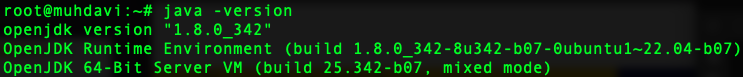
\includegraphics[width=\textwidth]{java-version}
\caption{Versi Java yang Terinstall}
\label{gam:java-version}
\end{figure}

\item Download Apache Hadoop \\
{\tt wget https://dlcdn.apache.org/hadoop/common/hadoop-3.3.4/hadoop-3.3.4.tar.gz}

\item Ekstrak Apache Hadoop \\
{\tt tar -xzvf hadoop-3.3.4.tar.gz }
\begin{itemize}
\item x $\Rightarrow$ ekstrak file arsip.
\item z $\Rightarrow$ filter file arsip melalui gzip.
\item v $\Rightarrow$ menampilkan proses.
\item f $\Rightarrow$ nama file arsip.
\end{itemize}

\item Pindahkan hasil ekstrak ke /usr/local/ \\
{\tt sudo mv hadoop-3.3.4 /usr/local/hadoop}

\item Edit file hadoop-env.sh dengan mengubah variabel JAVA\_HOME\footnote{Lebih jelasnya lihat Gambar \ref{gam:java-hadoop}} \\
{\tt cd /usr/local/hadoop} \\
{\tt sudo nano etc/hadoop/hadoop-env.sh} \\
\begin{lstlisting}
export JAVA\_HOME=/usr/lib/jvm/java-8-openjdk-amd64
\end{lstlisting}
\begin{figure}[!ht]
\centering
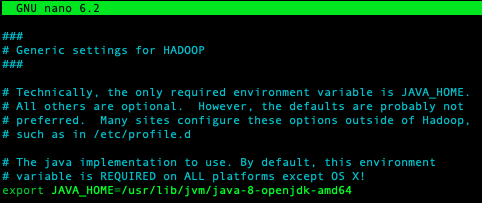
\includegraphics[width=.66\textwidth]{java-hadoop}
\caption{Konfigurasi Java Home}
\label{gam:java-hadoop}
\end{figure}

\item Menambahkan Hadoop Path ke {\tt .bashrc}\footnote{Lebih jelasnya lihat Gambar \ref{gam:hadoop-patch}} \\
{\tt sudo nano $\sim$/.bashrc} \\
\begin{lstlisting}
export HADOOP_HOME=/usr/local/hadoop
export HADOOP_CONF_DIR=${HADOOP_HOME}/etc/hadoop
export HADOOP_MAPRED_HOME=${HADOOP_HOME}
export HADOOP_COMMON_HOME=${HADOOP_HOME}
export HADOOP_HDFS_HOME=${HADOOP_HOME}
export YARN_HOME=${HADOOP_HOME}
export PATH=$PATH:/usr/local/hadoop/bin
\end{lstlisting}
{\tt source .bashrc}
\begin{figure}[!ht]
\centering
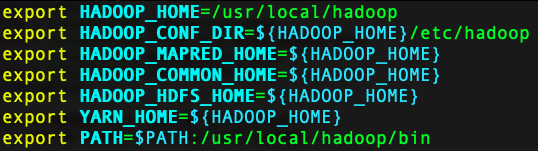
\includegraphics[width=\textwidth]{hadoop-path}
\caption{Konfigurasi Hadoop Path}
\label{gam:hadoop-path}
\end{figure}

\item Verifikasi Hasil Instalasi Hadoop \\
{\tt hadoop version} \\
Jika instalasi hadoop sudah berhasil, maka ketika mengecek versi hadoop akan muncul seperti yang diperlihatkan pada Gambar \ref{gam:hadoop-version}.
\begin{figure}[!ht]
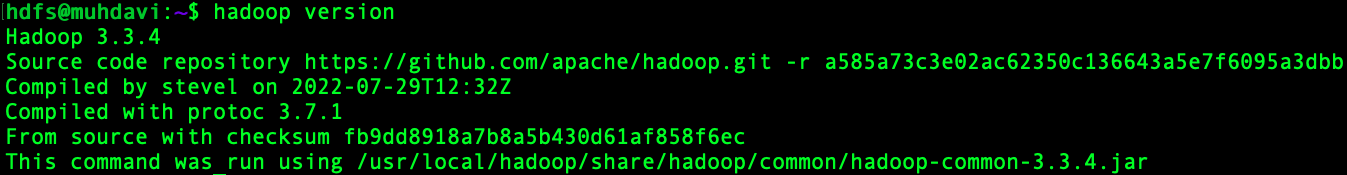
\includegraphics[width=\textwidth]{hadoop-version}
\caption{Versi Hadoop yang Terinstall}
\label{gam:hadoop-version}
\end{figure}
\end{enumerate}
 
\hrulefill

%%%%%%%%%%%%%%%%%%%%%%%%%%%%%%%%%%%%%%%%%%%%%%%%%%%%%%%%
\clearpage
\newday{22 September 2022}
\textit{N.B.: Setiap mahasiswa membuat laporan hasil praktik sesuai dengan format yang telah ditentukan. Template laporan dapat di download pada alamat \url{https://github.com/muhdavi/laporan-practice-big-data}.}

\newthought{Konfigurasi Apache Hadoop} \\
Setelah selesai meng-install Hadoop, kita perlu konfigurasi beberapa file Hadoop agar memudahkan kita dalam memonitoring ekosistem Hadoop yang telah diinstall.
\begin{enumerate}
\item Konfigurasi File Hadoop \\
File-file konfigurasi hadoop berada pada folder {\tt hadoop/etc/hadoop} seperti yang diperlihatkan pada Gambar \ref{gam:file-hadoop}.
{\tt cd /usr/local/hadoop/etc/hadoop} \\
{\tt ls}
\begin{figure}[!ht]
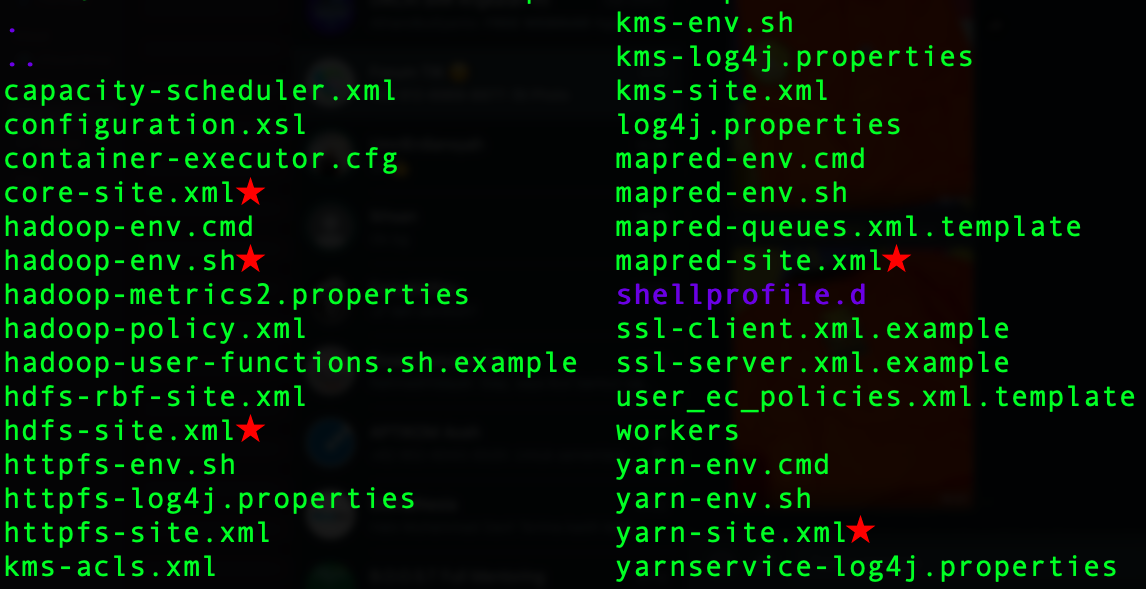
\includegraphics[width=\textwidth]{file-hadoop}
\caption{File Konfigurasi Hadoop}
\label{gam:file-hadoop}
\end{figure}

Beberapa file yang perlu dikonfigurasi adalah sebebai berikut:
\begin{itemize}
\item core-site.xml
\begin{lstlisting}
<property>
<name>fs.default.name</name>
<value>hdfs://localhost:9000</value>
</property>
\end{lstlisting}
\begin{figure}[!ht]
\centering
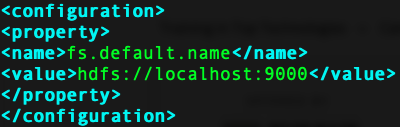
\includegraphics[width=.8\textwidth]{site-core}
\caption{Konfigurasi Core Site}
\label{gam:site-yarn}
\end{figure}

\item hdfs-site.xml
\begin{lstlisting}
<property>
<name>dfs.replication</name>
<value>1</value>
</property>
<property>
<name>dfs.permission</name>
<value>false</value>
</property>
\end{lstlisting}
\begin{figure}[!ht]
\centering
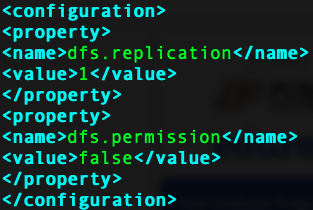
\includegraphics[width=.7\textwidth]{site-hdfs}
\caption{Konfigurasi HDFS Site}
\label{gam:site-yarn}
\end{figure}

\item mapred-site.xml
\begin{lstlisting}
<property>
<name>mapreduce.framework.name</name>
<value>yarn</value>
</property>
\end{lstlisting}
\begin{figure}[!ht]
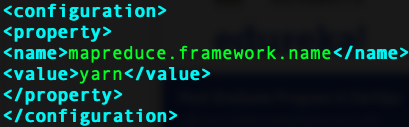
\includegraphics[width=\textwidth]{site-mapred}
\caption{Konfigurasi Mapred Site}
\label{gam:site-yarn}
\end{figure}

\item yarn-site.xml
\begin{lstlisting}
<property>
<name>yarn.nodemanager.aux-services</name>
<value>mapreduce_shuffle</value>
</property>
<property>
<name>
yarn.nodemanager.auxservices.mapreduce.shuffle.class
</name>
<value>org.apache.hadoop.mapred.ShuffleHandler</value>
</property>
\end{lstlisting}
\begin{figure}[!ht]
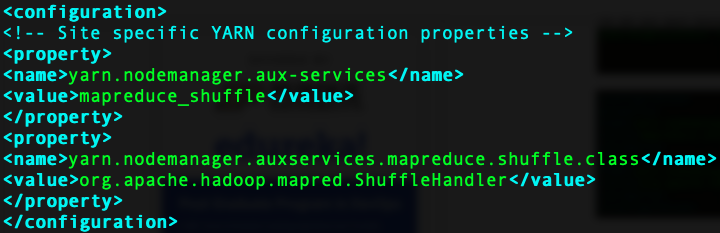
\includegraphics[width=\textwidth]{site-yarn}
\caption{Konfigurasi Yarn Site}
\label{gam:site-yarn}
\end{figure}
\end{itemize}

\item Jalankan Perintah Format Filesystem \\
{\tt hdfs namenode -format}
\begin{figure}[!ht]
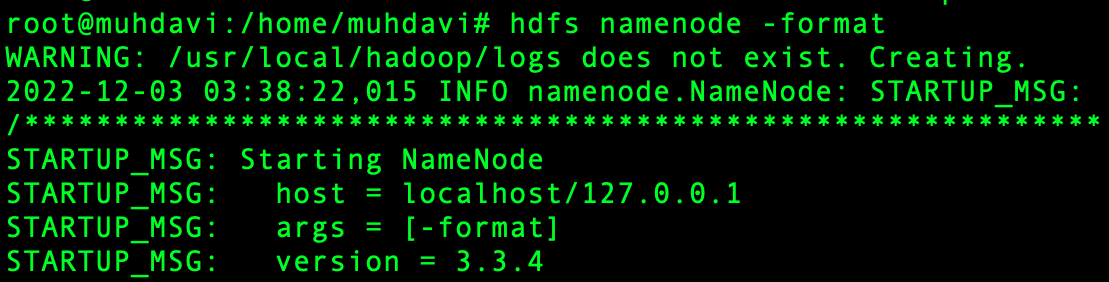
\includegraphics[width=\textwidth]{format-filesystem}
\caption{Format Filesystem}
\label{gam:format-filesystem}
\end{figure}

\item Jalankan NameNode Daemon dan DataNode Daemon \\
{\tt sbin/start-dfs.sh} \\
NameNode dapat diakses melalui \url{http://localhost:9870} dan akan tampil halaman web seperti yang diperlihatkan pada Gambar \ref{gam:namenode}.
\begin{figure}[!ht]
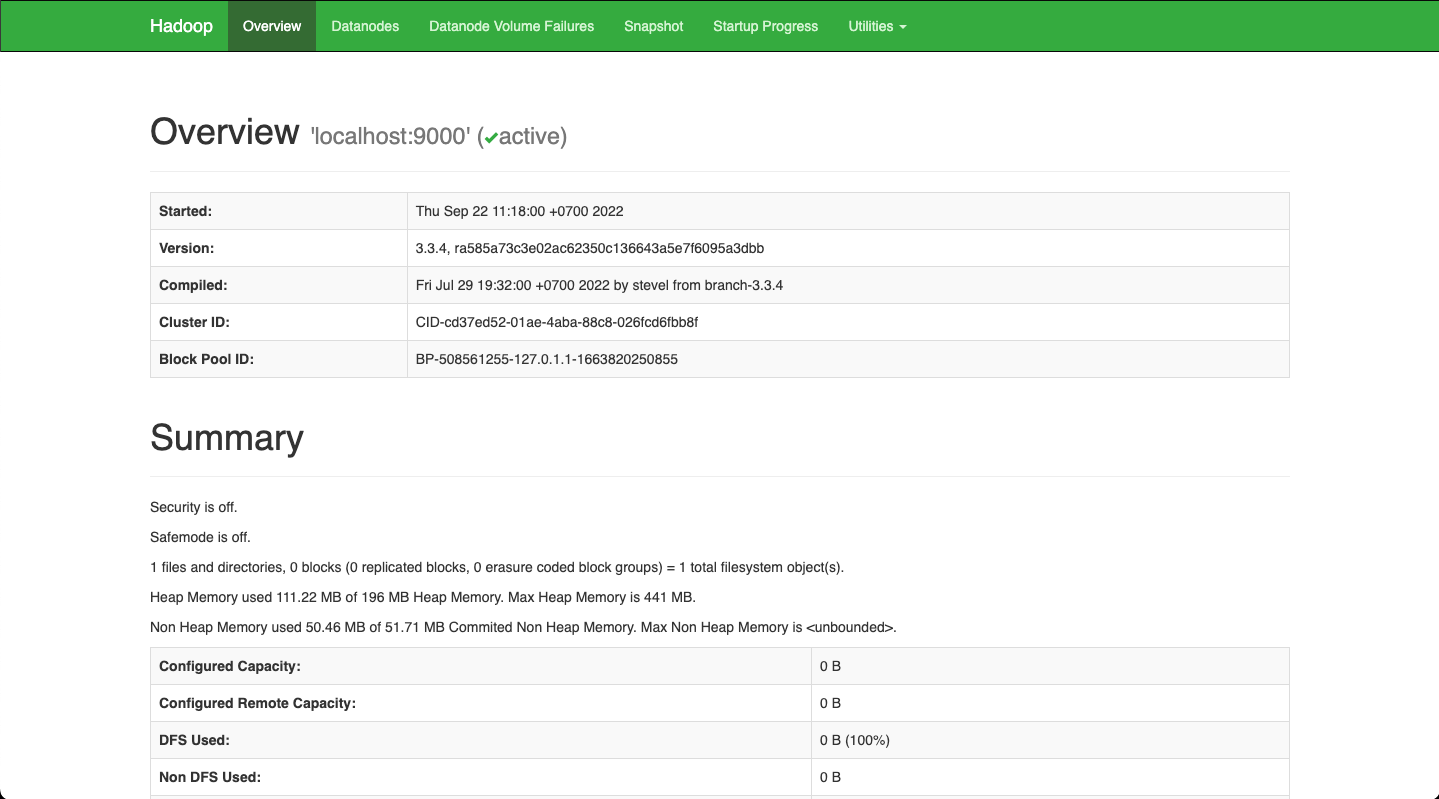
\includegraphics[width=\textwidth]{namenode}
\caption{Namemnode Hadoop}
\label{gam:namenode}
\end{figure}

\item Jalankan ResourceManager Daemon and NodeManager Daemon \\
{\tt sbin/start-yarn.sh} \\
ResourceManager dapat diakses melalui \url{http://localhost:8088} dan akan tampil halaman web serperti pada Gambar \ref{gam:namenode}.
\begin{figure}[!ht]
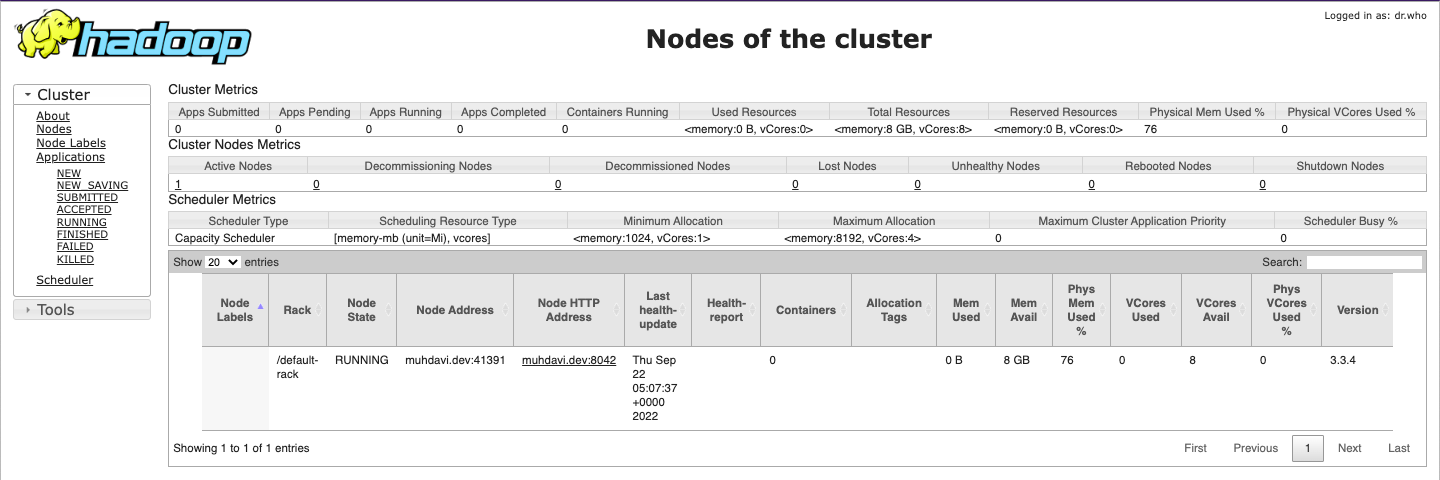
\includegraphics[width=\textwidth]{resourcemanager}
\caption{Resource Manager Hadoop}
\label{gam:resourcemanager}
\end{figure}
\end{enumerate}

\section{Laporan Mahasiswa}
\begin{enumerate}
\item Nadzura Kumaira		\\
\textit{isi laporan memuat langkah-langkah yang dilakukan, error dan hasil praktik.}
\item Nurani Harum Fardaniah\\
\textit{isi laporan memuat langkah-langkah yang dilakukan, error dan hasil praktik.}
\item Nuraula Tafiza		\\
\textit{isi laporan memuat langkah-langkah yang dilakukan, error dan hasil praktik.}
\item Nurul Aflah			\\
\textit{isi laporan memuat langkah-langkah yang dilakukan, error dan hasil praktik.}
\item Faiza Yuwafiqi		\\
\textit{isi laporan memuat langkah-langkah yang dilakukan, error dan hasil praktik.}
\item Adinda Awaliah		\\
\textit{isi laporan memuat langkah-langkah yang dilakukan, error dan hasil praktik.}
\item Adjie Yusmunandar		\\
\textit{isi laporan memuat langkah-langkah yang dilakukan, error dan hasil praktik.}
\item Arya Saputra			\\
\textit{isi laporan memuat langkah-langkah yang dilakukan, error dan hasil praktik.}
\item Jihan Dwi Sarah		\\
\textit{isi laporan memuat langkah-langkah yang dilakukan, error dan hasil praktik.}
\item Muhammad Munawir		\\
\textit{isi laporan memuat langkah-langkah yang dilakukan, error dan hasil praktik.}
\item Muhammad Ikrammullah	\\
\textit{isi laporan memuat langkah-langkah yang dilakukan, error dan hasil praktik.}
\item M. Ikhsan				\\
\textit{isi laporan memuat langkah-langkah yang dilakukan, error dan hasil praktik.}
\item Zulfahmi				\\
\textit{isi laporan memuat langkah-langkah yang dilakukan, error dan hasil praktik.}
\item Salsabila Irmanda		\\
\textit{isi laporan memuat langkah-langkah yang dilakukan, error dan hasil praktik.}
\item Siti Hajar Al Zahra	\\
\textit{isi laporan memuat langkah-langkah yang dilakukan, error dan hasil praktik.}
\item Syarfani Akbar		\\
\textit{isi laporan memuat langkah-langkah yang dilakukan, error dan hasil praktik.}
\item Cut Opy Mandalisa		\\
\textit{isi laporan memuat langkah-langkah yang dilakukan, error dan hasil praktik.}
\item Rauzatinur Syah		\\
\textit{isi laporan memuat langkah-langkah yang dilakukan, error dan hasil praktik.}
\item Resha Russita			\\
\textit{isi laporan memuat langkah-langkah yang dilakukan, error dan hasil praktik.}
\item Rizki Ilhami			\\
\textit{isi laporan memuat langkah-langkah yang dilakukan, error dan hasil praktik.}
\item Taravia Fauzah		\\
\textit{isi laporan memuat langkah-langkah yang dilakukan, error dan hasil praktik.}
\end{enumerate}

\hrulefill

%%%%%%%%%%%%%%%%%%%%%%%%%%%%%%%%%%%%%%%%%%%%%%%%%%%%%%%%


\newpage
\bibliographystyle{plain}
\bibliography{lab_notes}

\end{document}

\begin{comment}
\clearpage
\newday{22 September 2022}
\textit{N.B.: Setiap mahasiswa membuat laporan hasil praktikum dengan format yang telah ditentukan. Template laporan dapat di download pada alamat \url{https://github.com/muhdavi/laporan-practice-big-data}.}

\newthought{Konfigurasi Apache Hadoop} \\
\begin{figure}
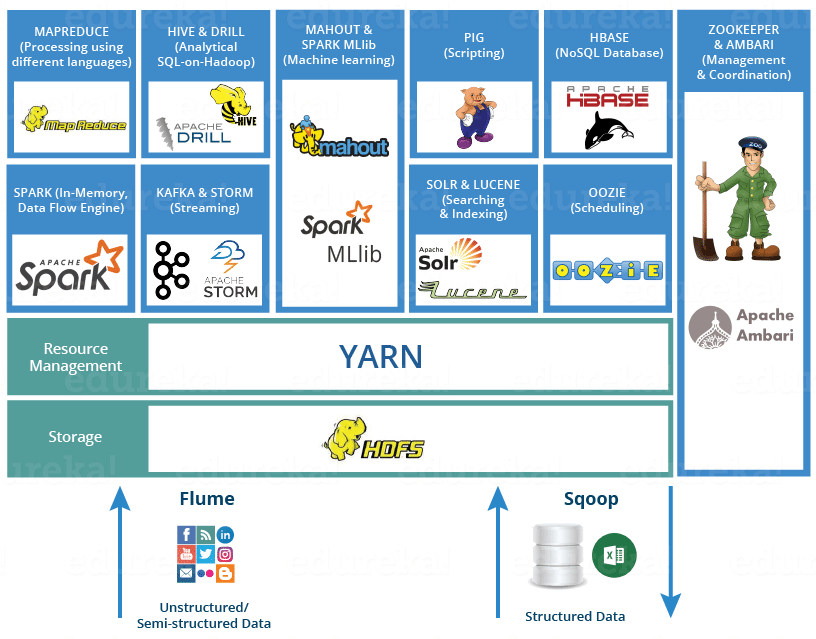
\includegraphics[width=\textwidth]{hadoop-ecosystem}
\caption{Ekosistem Hadoop}
\label{gam:hadoop-ecosystem}
\end{figure}
Seperti yang telah dibahas pada pertemuan sebelumnya bahwa Hadoop memiliki ekosistem sendiri dalam praktik big data seperti yang ditampilkan pada Gambar \ref{gam:hadoop-ecosystem}.

\hrulefill

%%%%%%%%%%%%%%%%%%%%%%%%%%%%%%%%%%%%%%%%%%%%%%%%%%%%%%%%

\section{Laporan Mahasiswa}
\begin{enumerate}
\item Nadzura Kumaira		\\
\textit{isi laporan}
\item Nurani Harum Fardaniah\\
\textit{isi laporan}
\item Nuraula Tafiza		\\
\textit{isi laporan}
\item Nurul Aflah			\\
\textit{isi laporan}
\item Faiza Yuwafiqi		\\
\textit{isi laporan}
\item Adinda Awaliah		\\
\textit{isi laporan}
\item Adjie Yusmunandar		\\
\textit{isi laporan}
\item Arya Saputra			\\
\textit{isi laporan}
\item Jihan Dwi Sarah		\\
\textit{isi laporan}
\item Muhammad Munawir		\\
\textit{isi laporan}
\item Muhammad Ikrammullah	\\
\textit{isi laporan}
\item M. Ikhsan				\\
\textit{isi laporan}
\item Zulfahmi				\\
\textit{isi laporan}
\item Salsabila Irmanda		\\
\textit{isi laporan}
\item Siti Hajar Al Zahra	\\
\textit{isi laporan}
\item Syarfani Akbar		\\
\textit{isi laporan}
\item Cut Opy Mandalisa		\\
\textit{isi laporan}
\item Rauzatinur Syah		\\
\textit{isi laporan}
\item Resha Russita			\\
\textit{isi laporan}
\item Rizki Ilhami			\\
\textit{isi laporan}
\item Taravia Fauzah		\\
\textit{isi laporan}
\end{enumerate}
\end{comment}
